\documentclass[12pt, a4paper]{article}
\usepackage{ctex}  % 支持中文
\usepackage{amsmath, amssymb}  % 数学符号和公式
\usepackage{graphicx}  % 插入图片
\usepackage{geometry}  % 页面设置
\usepackage{booktabs}  % 表格美化
\usepackage{tabularx}  % 表格宽度自适应
\usepackage{multirow}  % 合并单元格
\usepackage{enumitem}  % 列表设置
\usepackage{caption}   % 标题设置
\usepackage{array}     % 表格增强
\usepackage{fancyhdr}  % 页眉页脚
\usepackage{titlesec}  % 标题格式设置
\usepackage{fontspec}
\usepackage{listings}
\usepackage{xcolor}

\usepackage[
  backend=bibtex,
  style=gb7714-2015,   % 使用中国国标格式,适合中文论文
  sorting=none         % 按引用顺序排序
]{biblatex}

\addbibresource{references.bib} % 参考文献配置

% 页面设置
\geometry{left=2.5cm, right=2.5cm, top=2.5cm, bottom=2.5cm}

% 重定义section格式为居中
\titleformat{\section}{\centering\Large\bfseries}{\thesection}{1em}{}
\titleformat{\subsection}{\normalsize\bfseries}{\thesubsection}{1em}{}
\titleformat{\subsubsection}{\normalsize\bfseries}{\thesubsubsection}{1em}{}

% 表格表头格式
\renewcommand{\thetable}{\arabic{section}.\arabic{table}}

% 设置表格标题格式:左对齐,中文带"表"字,表题加粗
\captionsetup[table]{
  labelsep=space,
  labelformat=simple,
  textfont=bf,
  labelfont=bf,
  name=表
}

% 图片编号格式
\renewcommand{\thefigure}{\arabic{section}-\arabic{figure}}

% 设置图片标题格式
\captionsetup[figure]{
  labelsep=space,
  labelformat=simple,
  textfont=bf,     
  labelfont=bf, 
  position=bottom,  
  name=图
}

% 修改公式编号格式
\renewcommand{\theequation}{\thesection-\arabic{equation}}

% 参考文献格式
\makeatletter
\renewcommand\@biblabel[1]{[#1]}
\makeatother

% 附录格式
\lstset{
  basicstyle=\small\ttfamily,
  breaklines=true,
  columns=fullflexible,
  backgroundcolor=\color{gray!10},
  frame=single,
  rulecolor=\color{black!30},
  commentstyle=\color{green!50!black},
  keywordstyle=\color{blue},
  stringstyle=\color{red},
  numbers=left,
  numberstyle=\tiny\color{gray},
  numbersep=5pt
}


\begin{document}

% 标题部分
\begin{center}
\LARGE\textbf{深度学习与传统计量模型融合框架下的市场风险度量:LSTM-GARCH混合模型在A股VaR预测中的应用}

\vspace{1cm}
\large 计金220 22011854 高菻铠
\end{center}

\noindent \textbf{摘要:} 本文构建了一个融合长短期记忆网络与广义自回归条件异方差模型的混合框架,旨在提高中国A股市场风险价值的预测准确性。通过对上证综指1995-2025年日度数据的实证分析,研究发现:(1)A股市场收益率表现出显著的“尖峰厚尾”分布特征和波动聚集效应,考虑非对称效应和厚尾分布的GJR-GARCH(1,1)-t模型在传统方法中表现最佳;(2)在波动率预测方面,LSTM模型显著优于GARCH(1,1)-Normal模型,其均方根误差为0.0063,较后者降低56.2\%,反映了深度学习模型在捕捉复杂非线性依赖关系上的优势;(3)混合模型虽未在所有指标上超越单一模型,但提供了更为稳定且范围适中的预测,降低了极端预测风险;(4)在95\%置信水平下的VaR预测中,GARCH(1,1)-Normal模型的实际超越率0.0430最接近理论值0.05,而LSTM和混合模型表现出更为保守的风险估计。这一“悖论”表明,高精度的波动率预测未必直接转化为准确的VaR估计。研究结果对不同市场参与者的风险管理实践具有差异化价值,并为深度学习与传统计量模型的融合应用提供了新思路。本研究的全部代码可在此网址找到:\textbf{https://github.com/1517005260/stock-agent/blob/master/test/ml-garch-var.ipynb}。

\noindent \textbf{关键词:} 风险价值;LSTM-GARCH混合模型;波动率预测;深度学习;中国A股市场

\section{绪论}

金融市场风险度量对于投资者和监管机构而言始终是核心课题。在全球金融市场日益复杂化、波动性增强的背景下,准确预测市场风险不仅关系到投资决策的有效性,也直接影响着金融体系的稳定性。风险价值VaR作为衡量市场风险的主要工具,能够在给定置信水平下量化特定时间范围内可能发生的最大损失,已经成为监管部门和金融机构的标准风险度量方法。

传统上,广义自回归条件异方差GARCH模型自\citet{bollerslev1986generalized}提出以来,在金融波动率建模和风险度量领域发挥了重要作用。GARCH模型能够有效捕捉金融时间序列数据中的“波动率聚类”现象,即高波动性时期往往会聚集出现,而低波动性时期同样表现出聚集特性。\citet{wang2022practical}指出,GARCH模型虽然不能解释波动率聚类的内在原因,但其基于过去波动逐步衰减的建模方式能够准确描述上述特征。然而,随着金融市场复杂性的增加以及人工智能技术的发展,传统GARCH模型在处理高度非线性和复杂依赖关系的金融时间序列时逐渐显露不足。\citet{tsay2013financial}指出,传统的GARCH族模型往往需要较高的阶数才能有效捕捉复杂市场的波动特征,这不仅增加了模型的复杂性,还可能导致过拟合。

近年来,以深度学习为代表的人工智能技术在金融领域的应用日益广泛。\citet{hochreiter1997lstm}提出的长短期记忆网络LSTM通过其特殊的门控机制,有效解决了传统递归神经网络RNN中的梯度消失问题,为时间序列预测提供了更可靠的技术支持。\citet{yuan2020comprehensive}对金融市场预测中深度学习方法的全面调查表明,LSTM在股票价格预测中表现出色,特别是在充分考虑时间序列特性的情况下,能够捕捉复杂的时间依赖关系。\citet{sullivan2019stock}专门研究了LSTM网络在股票波动率预测中的应用,发现LSTM结构特别适合处理金融时间序列中“重要事件”间隔时间不均匀的特点,因为LSTM的“记忆”特性能够保持对旧数据点的影响。该研究还指出,金融时间序列的自相关性使得LSTM中的单元记忆在训练和测试网络时非常有用。

在中国市场的应用方面,\citet{cao2005nonlinear}的研究使用了367家在上海证券交易所交易的上市公司的日收盘价数据,比较了线性模型,如Fama-French模型,和神经网络的预测能力。研究结果表明,神经网络更适合预测像中国这样的新兴股票市场上交易的股票价格。另外,\citet{qiaoa2022prediction}基于2019年至2021年的上海和深圳股票市场数据,使用LSTM模型对股票收益率进行预测,采用滚动窗口方法在样本内优化和样本外测试,表明LSTM深度神经网络在预测中国股市方面是有效的,能够提高股票收益率的预测准确性。

随着研究的深入,学者们发现单一模型难以全面捕捉金融时间序列的特征,混合模型逐渐成为研究热点。\citet{kim2018forecasting}首次提出了将LSTM与多种GARCH型模型集成的混合方法来预测股价波动率。该研究使用韩国KOSPI 200指数数据构建了LSTM与一至三个GARCH型模型结合的混合模型,并与现有方法,包括单一模型如GARCH、EGARCH、EWMA、深度前馈神经网络和LSTM等,进行比较。研究发现,结合LSTM模型与三种GARCH型模型的GEW-LSTM混合模型在平均绝对误差MAE、均方误差MSE、异方差调整MAE和异方差调整MSE等多项指标上表现最佳。在中国市场,\citet{zhang2024vmd}研究了投资者情绪与股票指数之间的波动相关性,采用变分模态分解和长短期记忆VMD-LSTM,混合神经网络模型对投资者情绪指数和上海证券交易所综合指数进行分解和重构,将其分为短期、中期和长期趋势。通过GARCH模型和LSTM模型的结合,能够更好地捕捉中国股市投资者情绪与股价波动之间的关系。

VaR的预测是风险管理的核心任务之一,混合模型在VaR预测方面也展现出优势。\citet{kakade2022value}提出了一种新型混合模型,将LSTM和BiLSTM神经网络与GARCH型模型预测结合,使用集成学习方法预测一天后95\%和99\%置信水平下的VaR。该研究利用标准GARCH、EGARCH和门限GARCH模型的预测能力与LSTM网络相结合,捕捉底层波动率的不同特征。实证研究表明,混合模型在所有损失函数和覆盖率测试中均优于其他所有模型,显著提高了VaR预测的质量和准确性。\citet{firdous2023garch}提出了GARCH-MIDAS-LSTM模型,融合了LSTM深度神经网络和GARCH-MIDAS模型的优势。该模型在市场波动较大的时期的样本内建模和样本外预测方面均表现优异。

近期研究不断在LSTM-GARCH混合模型基础上进行创新。\citet{araya2024hybrid}研发了结合GARCH簇模型、XGBoost算法和LSTM网络的混合模型用于预测波动率。实证研究表明,LSTM在标准普尔500指数和苹果公司的预测中显著优于GARCH模型。\citet{yao2024time}研究了中国A股指数的预测,采用先动态分离、再预测、最后合并的方法,提高了预测准确性并避免了过度数据挖掘。\citet{chen2024hybrid}提出了一种结合完全集成经验模态分解CEEMD、Time2Vec和Transformer的新型模型,以更好地捕捉和利用股票数据中的各种模式。

尽管现有研究取得了显著进展,但在中国A股市场风险度量领域,尤其是VaR预测方面,深度学习与传统计量模型融合方法的应用仍然较为有限。中国A股市场作为一个快速发展的新兴市场,具有独特的市场特征和波动模式。A股市场的交易限制,例如涨跌停板制度、投资者结构以散户为主以及政策敏感性,都使得其波动特性与成熟市场存在显著差异。此外,中国资本市场开放程度不断提高,全球金融市场波动的溢出效应也对A股市场风险产生了重要影响。这些因素共同构成了A股市场波动率和风险预测的复杂背景,对预测模型提出了更高的要求。

本研究的目的在于探索深度学习与传统计量模型融合框架下的市场风险度量方法,即LSTM-GARCH混合模型在A股VaR预测中的应用。与现有研究相比,本文的创新之处主要体现在以下几个方面:首先,本研究针对中国A股市场的特殊性,设计了适合捕捉A股波动特征的LSTM-GARCH混合模型架构;其次,通过引入多维特征工程,增强了模型对市场微观结构和宏观经济环境变化的敏感性;第三,提出了基于滚动窗口的动态权重调整机制,使混合模型能够根据市场状态自适应调整LSTM与GARCH的权重分配,从而在不同市场环境下保持稳定的预测性能;最后,建立了一套基于VaR预测准确性的综合评估框架,全面评价混合模型的风险预测能力。

本研究的理论意义在于丰富和深化了金融市场风险度量的方法论体系,为混合模型在新兴市场风险管理中的应用提供了新的思路和实证证据。从实践角度看,本研究开发的LSTM-GARCH混合模型可为金融机构风险管理、投资决策以及监管部门的市场风险评估提供更为准确的量化工具,有助于提高市场参与者的风险识别能力,促进中国资本市场的稳定发展。

本文的结构安排如下:第一章为绪论,介绍研究背景、文献综述和研究意义;第二章为问题描述,阐述研究问题和挑战;第三章为数学建模,详细描述了模型的数学框架;第四章为数值求解,提供了数据分析和模型评估结果;第五章为结果讨论,深入分析实证发现;第六章为结论,总结研究成果并指出未来研究方向。

\section{问题描述}

市场交易机制、投资者结构以及政策敏感性等,共同塑造了A股市场波动性的独特模式。这些特征使得A股市场的风险表现出与成熟市场不同的动态特性,为风险度量带来了特殊挑战。VaR作为巴塞尔协议推荐的标准风险度量工具,其在A股市场的准确预测对于金融机构风险管理和监管政策制定具有重要意义。

从技术层面看,VaR是在给定置信水平$1-\alpha$下,未来$h$个交易日内可能发生的最大预期损失。对金融机构而言,VaR是资本充足率计算、交易限额设定和风险敞口管理的基础。随着中国金融市场的对外开放和监管体系的完善,银保监会和证监会逐步强化了市场风险管理要求,使VaR日益成为中国金融机构风险控制的核心工具。

传统的VaR预测方法虽然各有优势,但在应对A股市场的复杂性时也暴露出局限:GARCH簇模型虽能有效捕捉波动率聚类,但其线性结构难以适应市场结构性变化;历史模拟法过于依赖历史数据的代表性;蒙特卡洛模拟法则高度依赖于分布假设的准确性。深度学习模型如LSTM网络等虽能识别复杂的非线性模式和长期依赖关系,但在短期波动建模和可解释性方面存在不足。

本研究的核心问题在于:如何构建一个融合GARCH模型与LSTM网络优势的混合框架,以更准确地预测A股市场的风险价值。具体而言,研究需要解决以下关键问题:一是混合架构的设计,使GARCH模型在短期波动建模的优势与LSTM在复杂非线性关系捕捉上的能力相互补充;二是特征工程的优化,以反映A股市场微观结构和宏观环境信息;三是权重机制的建立,合理分配LSTM与传统GARCH模型的比重;四是建立完善的评估体系,关注极端市场条件下的预测表现。这些问题的有效解决将为A股市场风险管理提供更精准的量化工具。

\section{数学建模}

本研究构建的LSTM-GARCH混合模型框架涉及三个主要组成部分:波动率预测模型、特征工程和风险价值计算。以下将详细阐述各部分的数学建模过程。

首先,金融资产的对数收益率是波动率建模的基础,对于股票指数或个股价格序列$P_t$,其对数收益率$r_t$定义为:

\begin{equation}
r_t = \ln\left(\frac{P_t}{P_{t-1}}\right)
\end{equation}

基于对数收益率序列,GARCH模型描述了波动率的时变特性。在本研究中,我们采用GJR-GARCH(1,1)模型来捕捉A股市场中常见的波动率非对称效应(即负向冲击对波动率的影响大于正向冲击),模型设定如下:

\begin{equation}
r_t = \mu + \varepsilon_t
\end{equation}

\begin{equation}
\varepsilon_t = \sigma_t z_t, \quad z_t \sim F(0,1)
\end{equation}

\begin{equation}
\sigma_t^2 = \omega + \alpha\varepsilon_{t-1}^2 + \gamma I_{t-1}\varepsilon_{t-1}^2 + \beta\sigma_{t-1}^2
\end{equation}

其中,$\mu$为条件均值,$\varepsilon_t$为随机扰动项,$\sigma_t^2$为条件方差,$z_t$为服从标准化分布$F$的随机变量,$I_{t-1}$为指示函数,当$\varepsilon_{t-1} < 0$时取值为1,否则为0。参数$\alpha$衡量过去冲击对当前波动率的影响,$\gamma$捕捉非对称效应,$\beta$度量波动率的持续性。当$\gamma > 0$时,表明负向冲击对波动率的影响大于正向冲击,这一现象在A股市场中尤为明显。

为了增强对长期依赖关系和非线性模式的捕捉能力,本研究引入了基于LSTM的深度学习模型。LSTM单元的核心在于其能够通过门控机制选择性地记忆和遗忘信息,有效解决传统RNN中的梯度消失问题。LSTM单元的数学表达如下:

\begin{equation}
f_t = \sigma(W_f \cdot [h_{t-1}, x_t] + b_f)
\end{equation}

\begin{equation}
i_t = \sigma(W_i \cdot [h_{t-1}, x_t] + b_i)
\end{equation}

\begin{equation}
\tilde{C}_t = \tanh(W_C \cdot [h_{t-1}, x_t] + b_C)
\end{equation}

\begin{equation}
C_t = f_t \odot C_{t-1} + i_t \odot \tilde{C}_t
\end{equation}

\begin{equation}
o_t = \sigma(W_o \cdot [h_{t-1}, x_t] + b_o)
\end{equation}

\begin{equation}
h_t = o_t \odot \tanh(C_t)
\end{equation}

其中,$f_t$、$i_t$和$o_t$分别为遗忘门、输入门和输出门,$C_t$为细胞状态,$h_t$为隐藏状态,$x_t$为时间$t$的输入特征向量,$W_f$、$W_i$、$W_C$和$W_o$为权重矩阵,$b_f$、$b_i$、$b_C$和$b_o$为偏置向量,$\sigma$为sigmoid激活函数,$\tanh$为双曲正切激活函数,$\odot$表示Hadamard乘积(元素级乘法)。

在本研究中,LSTM模型的输入特征$x_t$包含多维市场信息,不仅包括历史收益率和波动率,还包括反映市场微观结构和宏观环境的特征:

\begin{equation}
x_t = [r_t, r_{t-1}, ..., r_{t-n}, \sigma_t^{GARCH}, TR_t, VC_t, PV10_t, PV30_t, MS_t, ME_t]
\end{equation}

其中,$r_t, r_{t-1}, ..., r_{t-n}$为滞后$n$期的对数收益率,$\sigma_t^{GARCH}$为GARCH模型预测的条件波动率,$TR_t$为对数交易范围(日高低价之差的对数),$VC_t$为对数交易量变化,$PV10_t$和$PV30_t$分别为前10天和30天的历史波动率,$MS_t$为市场微观结构特征,$ME_t$为宏观经济指标。

LSTM模型的输出层设计为预测未来$h$天的波动率:

\begin{equation}
\hat{\sigma}_{t+1:t+h}^{LSTM} = W_o \cdot h_t + b_o
\end{equation}

在混合模型框架中,GARCH和LSTM的预测结果通过动态权重机制进行整合:

\begin{equation}
\hat{\sigma}_{t+1:t+h}^{Hybrid} = \lambda_t \cdot \hat{\sigma}_{t+1:t+h}^{LSTM} + (1 - \lambda_t) \cdot \hat{\sigma}_{t+1:t+h}^{GARCH}
\end{equation}

其中,$\lambda_t \in [0,1]$为动态权重,其值取决于当前市场状态:

\begin{equation}
\lambda_t = \sigma\left(W_{\lambda} \cdot [MS_t, PV30_t, ME_t] + b_{\lambda}\right)
\end{equation}

基于混合模型预测的波动率,我们计算给定置信水平$1-\alpha$下的风险价值(VaR):

\begin{equation}
VaR_{t+1:t+h}^{\alpha} = -(\mu_{t+1:t+h} + z_{\alpha} \cdot \hat{\sigma}_{t+1:t+h}^{Hybrid} \cdot \sqrt{h})
\end{equation}

其中,$\mu_{t+1:t+h}$为预测期内的预期收益率,$z_{\alpha}$为标准正态分布在置信水平$1-\alpha$下的分位数,$\sqrt{h}$为时间调整因子。

为了全面评估混合模型的VaR预测性能,我们采用多种统计检验方法。首先,通过计算实际超越次数与理论超越次数的比率,评估VaR预测的准确性:

\begin{equation}
Hit_t = I(r_t < -VaR_t^{\alpha})
\end{equation}

\begin{equation}
\hat{\alpha} = \frac{1}{T} \sum_{t=1}^{T} Hit_t
\end{equation}

理想情况下,$\hat{\alpha}$应接近于$\alpha$。我们使用Kupiec的覆盖率检验(POF检验)评估VaR模型的无条件覆盖性:

\begin{equation}
LR_{POF} = -2\ln\left[\frac{\alpha^x (1-\alpha)^{T-x}}{{\hat{\alpha}}^x (1-\hat{\alpha})^{T-x}}\right]
\end{equation}

其中,$x = \sum_{t=1}^{T} Hit_t$为总超越次数,$T$为样本量。该统计量在原假设下渐近服从自由度为1的卡方分布。

此外,我们还使用Christoffersen的条件覆盖率检验,评估VaR预测失败的独立性和覆盖率:

\begin{equation}
LR_{CC} = LR_{POF} + LR_{IND}
\end{equation}

其中,$LR_{IND}$为独立性检验统计量,检验VaR超越事件是否存在时间聚类。$LR_{CC}$在原假设下渐近服从自由度为2的卡方分布。

最后,我们采用Lopez损失函数评估不同模型预测VaR的整体性能:

\begin{equation}
L_t = \begin{cases}
1 + (r_t + VaR_t^{\alpha})^2, & \text{if } r_t < -VaR_t^{\alpha} \\
0, & \text{otherwise}
\end{cases}
\end{equation}

总损失为各期损失的累加:$L = \sum_{t=1}^{T} L_t$。Lopez损失函数不仅考虑了VaR超越的频率,还考虑了超越幅度,提供了更全面的性能评估。

通过上述数学建模框架,LSTM-GARCH混合模型充分考虑了A股市场的特殊性,引入了多维特征工程和动态权重调整机制,有望为金融机构和监管部门提供更为可靠的风险管理工具。

\section{数值求解}

针对前文所构建的LSTM-GARCH混合模型框架,本研究采用多步骤求解策略,通过数据预处理、特征构建、模型训练与评估等环节实现整体框架。全部实验均基于上证综指1995年至2025年的日度交易数据,样本包含7361个交易日,为确保模型的稳定性和可靠性,采用滚动窗口法进行模型训练与测试。

首先,对上证综指的原始价格序列进行处理,计算日度对数收益率,并检验其统计特性。图\ref{fig:sse_returns_ts}展示了上证综指的日收益率时间序列,可以直观观察到收益率序列呈现波动聚集特征,即高波动率和低波动率时期倾向于聚集出现。

\begin{figure}[htbp]
\centering
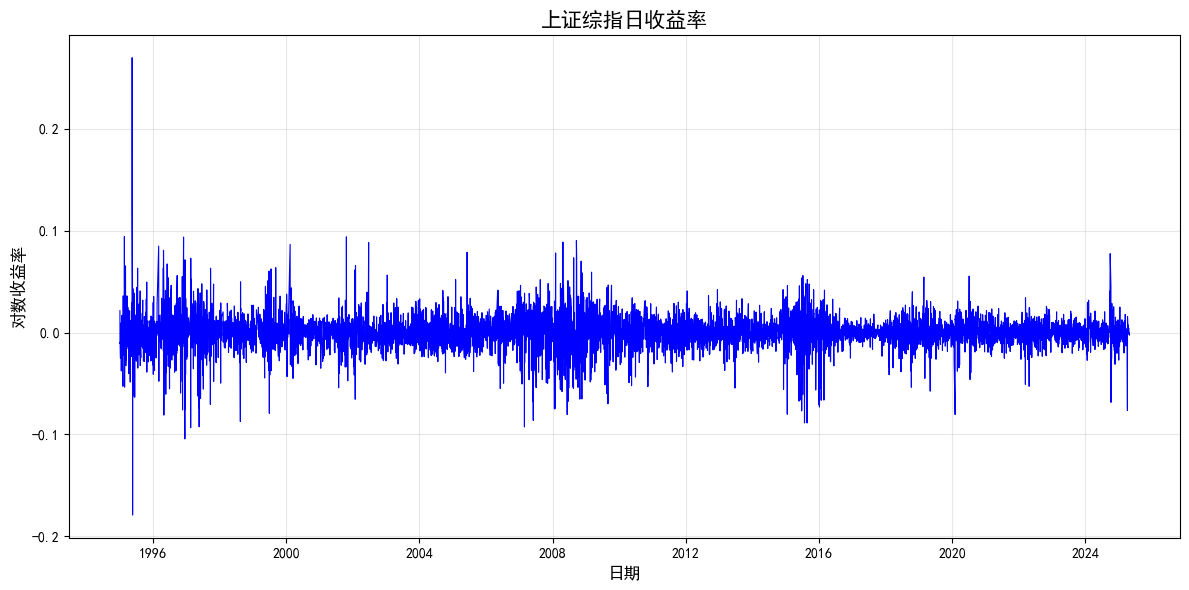
\includegraphics[width=0.8\textwidth]{./img/上证综指日收益率.png}
\caption{上证综指日收益率时间序列(1995-2025)}
\label{fig:sse_returns_ts}
\end{figure}

表\ref{tab:sse_stats}列出了上证综指日收益率的描述性统计结果。数据显示收益率序列均值接近于零,表现出0.1597的正偏度和显著的尖峰特征(峰度为17.01),这意味着收益率分布相较于正态分布具有更高的中心峰值和更厚的尾部。Jarque-Bera检验的显著p值进一步证实了收益率分布的非正态性。同时,ADF检验的p值为3.69e-24,非常显著,表明收益率序列是平稳的,为后续的时间序列建模奠定了基础。

\begin{table}[htbp]
\centering
\caption{上证综指日收益率描述性统计(1995-2025)}
\label{tab:sse_stats}
\begin{tabular}{lc}
\toprule
统计量 & 数值 \\
\midrule
观测值 & 7,361 \\
均值 & 2.22e-04 \\
中位数 & 4.70e-04 \\
标准差 & 1.64e-02 \\
偏度 & 0.1597 \\
峰度 & 17.0087 \\
最小值 & -0.1791 \\
最大值 & 0.2693 \\
Jarque-Bera统计量 & 88,631.84 \\
J-B p值 & 0.0000 \\
ADF统计量 & -12.9318 \\
ADF p值 & 3.69e-24 \\
\bottomrule
\end{tabular}
\end{table}

图\ref{fig:sse_returns_dist}呈现了收益率的分布特征与Q-Q图。直方图显示收益率分布相较于正态分布具有更高的峰值和更厚的尾部,Q-Q图则进一步确认了分布的非正态性,特别是在尾部区域的偏离更为明显。这些特征表明,传统假设正态分布的风险度量方法可能低估市场极端风险。

\begin{figure}[htbp]
\centering
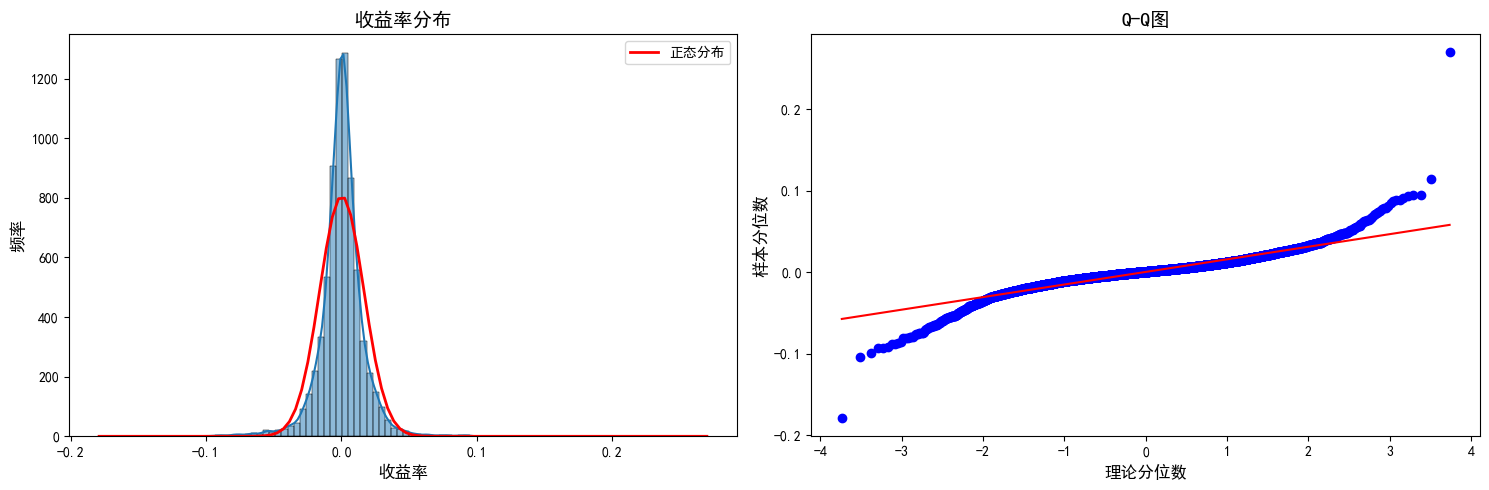
\includegraphics[width=0.8\textwidth]{./img/收益率分布.png}
\caption{上证综指日收益率分布与Q-Q图}
\label{fig:sse_returns_dist}
\end{figure}

针对收益率序列的波动特性,本研究首先进行ARCH效应检验。表\ref{tab:arch_effect}展示了在不同滞后阶数下的ARCH-LM检验结果,所有滞后阶数下p值均为0,强烈拒绝了“不存在ARCH效应”的原假设,证实了上证综指收益率序列存在显著的异方差特性,这支持了采用GARCH类模型进行波动率建模的合理性。

\begin{table}[htbp]
\centering
\caption{ARCH效应检验结果}
\label{tab:arch_effect}
\begin{tabular}{ccc}
\toprule
滞后阶数 & LM统计量 & p值 \\
\midrule
1 & 196.36 & 1.30e-44 \\
5 & 838.13 & 6.51e-179 \\
10 & 867.10 & 7.65e-180 \\
\bottomrule
\end{tabular}
\end{table}

基于上述分析,本研究首先建立传统的GARCH模型系列,包括GARCH(1,1)-Normal、GARCH(1,1)-t、GJR-GARCH(1,1)-Normal和GJR-GARCH(1,1)-t四种规格,通过信息准则和残差诊断选择最优模型。表\ref{tab:garch_models}展示了四种GARCH模型的比较结果。

\begin{table}[htbp]
\centering
\caption{GARCH模型比较结果}
\label{tab:garch_models}
\begin{tabular}{lcccc}
\toprule
模型 & Log-Likelihood & AIC & BIC & LB-Q²(10) \\
\midrule
GARCH(1,1)-Normal & 21,020.7 & -42,031.4 & -41,996.8 & 0.0000 \\
GARCH(1,1)-t & 21,256.3 & -42,500.6 & -42,459.3 & 0.0023 \\
GJR-GARCH(1,1)-Normal & 21,143.1 & -42,274.2 & -42,232.9 & 0.0012 \\
GJR-GARCH(1,1)-t & 21,321.8 & -42,629.6 & -42,581.7 & 0.0687 \\
\bottomrule
\end{tabular}
\end{table}

根据AIC和BIC信息准则以及残差诊断结果,GJR-GARCH(1,1)-t模型表现最佳,这表明考虑了波动率的非对称的杠杆效应和较厚尾部分布的模型更适合描述上证综指的波动特性。图\ref{fig:garch_cond_vol}展示了GARCH(1,1)-Normal估计的条件波动率序列,可以清晰观察到市场波动率的时变特性,特别是在1996年、2008年和2015年等市场危机或剧烈调整时期的高波动现象。

\begin{figure}[htbp]
\centering
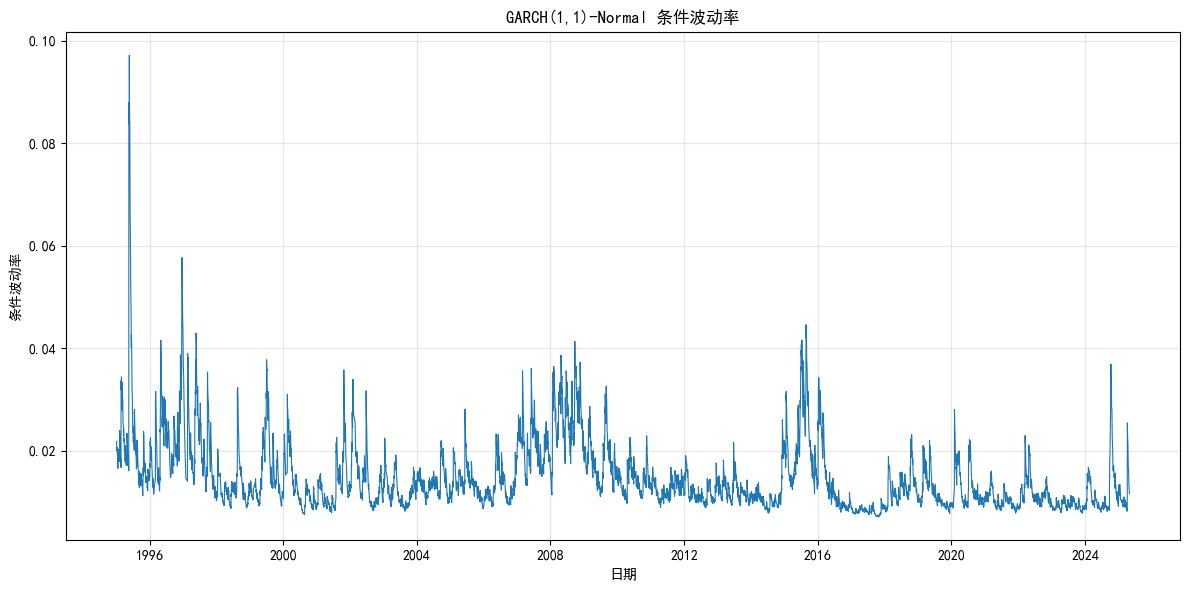
\includegraphics[width=0.8\textwidth]{./img/GARCH条件波动率.png}
\caption{GARCH(1,1)-Normal模型条件波动率}
\label{fig:garch_cond_vol}
\end{figure}

图\ref{fig:garch_std_resid}呈现了GARCH模型标准化残差的分析结果。从时间序列图和自相关图来看,标准化残差基本呈现随机性,不存在明显的序列相关性,表明GARCH模型较好地捕捉了收益率序列的条件异方差特性。然而,从分布直方图和Q-Q图可以观察到,即使在考虑t分布的情况下,标准化残差的尾部行为仍有偏离,表示可能存在GARCH模型难以捕捉的非线性特征。

\begin{figure}[htbp]
\centering
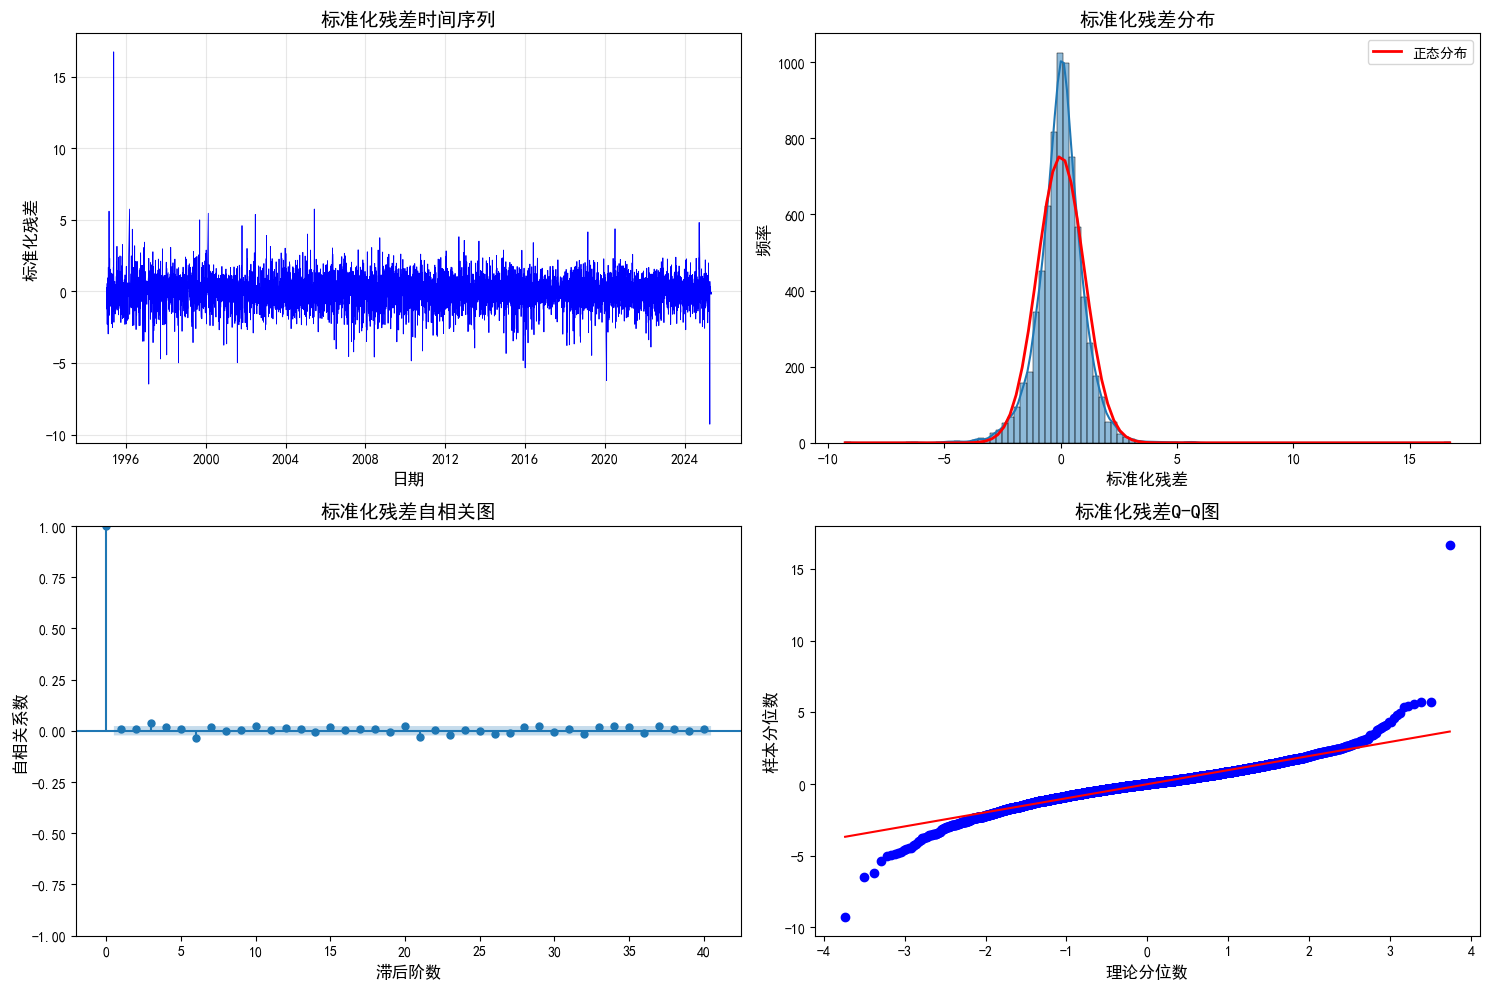
\includegraphics[width=0.8\textwidth]{./img/标准化残差分析.png}
\caption{GARCH模型标准化残差分析}
\label{fig:garch_std_resid}
\end{figure}

在GARCH模型的基础上,本研究构建了基于LSTM的深度学习模型。在特征工程阶段,我们不仅包含了传统的技术指标,如历史收益率、交易量变化和历史波动率,还引入了GARCH预测波动率作为重要特征,从而实现两种模型框架的初步融合。模型采用30天的滚动窗口作为输入,预测未来10天的平均波动率。LSTM网络结构包含两个LSTM层,每层200个单元,通过dropout机制(比率为0.1)防止过拟合。训练采用Adam优化器,批量大小为700,学习率为0.01,训练轮次为60。

图\ref{fig:lstm_train_loss}展示了LSTM模型的训练损失曲线。从曲线可以观察到,模型损失在前10个epoch迅速下降,之后进入相对平稳阶段,并在40-50epoch之间出现小幅波动,最终在第60个epoch达到0.0166的稳定损失值。训练过程表明模型成功学习了数据中的模式,同时没有出现显著的过拟合现象。

\begin{figure}[htbp]
\centering
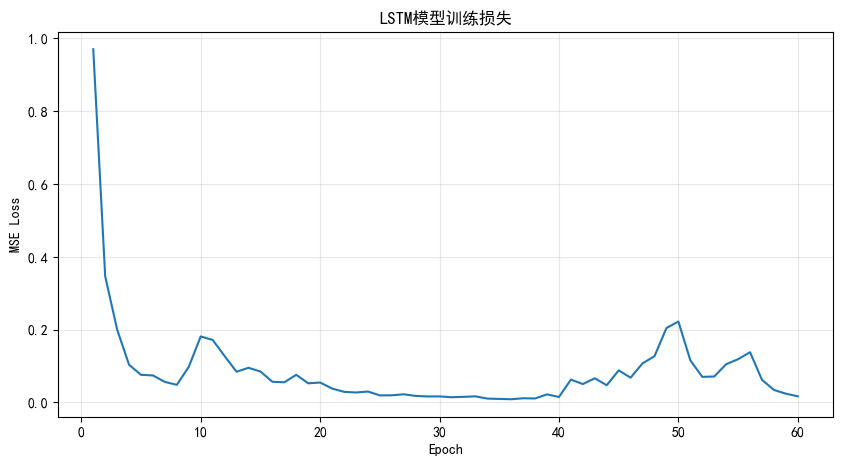
\includegraphics[width=0.8\textwidth]{./img/LSTM训练损失.png}
\caption{LSTM模型训练损失曲线}
\label{fig:lstm_train_loss}
\end{figure}

在单独评估GARCH和LSTM模型性能的基础上,本研究构建了LSTM-GARCH混合模型。混合模型采用动态权重机制,根据市场状态自适应调整两个模型的贡献比例。图\ref{fig:vol_pred_compare}展示了三种模型在测试集前100个样本上的波动率预测比较,可以观察到GARCH模型在低波动期间倾向于低估波动率,而在高波动期间反应不足;LSTM模型能够更好地捕捉波动的变化趋势,但在极端波动期间存在滞后;混合模型则兼具两者优势,在保持对波动趋势敏感性的同时,提供了更为平滑和稳健的预测。

\begin{figure}[htbp]
\centering
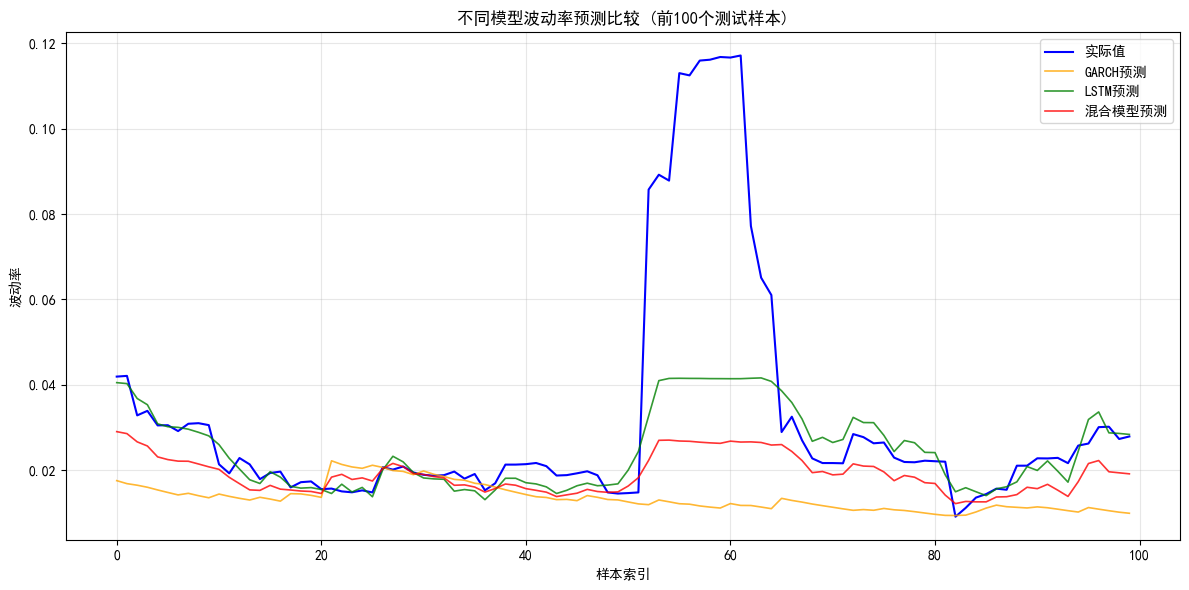
\includegraphics[width=0.8\textwidth]{./img/不同模型波动率预测比较.png}
\caption{不同模型波动率预测比较 (前100个测试样本)}
\label{fig:vol_pred_compare}
\end{figure}

表\ref{tab:vol_metrics}列出了三种模型在波动率预测方面的性能指标。结果显示,LSTM模型在MSE、RMSE、MAE和R²等多个指标上均优于GARCH(1,1)-Normal模型,表明深度学习模型在捕捉上证综指波动特征方面具有显著优势。混合模型虽然在某些指标上未能超越单独的LSTM模型,但R²值显著高于GARCH模型,表明其综合预测能力仍然较强。

\begin{table}[htbp]
\centering
\caption{不同模型波动率预测性能比较}
\label{tab:vol_metrics}
\begin{tabular}{lcccc}
\toprule
模型 & MSE & RMSE & MAE & R² \\
\midrule
GARCH(1,1)-Normal & 0.000206 & 0.014349 & 0.008985 & -0.332235 \\
LSTM & 0.000040 & 0.006287 & 0.002215 & 0.744265 \\
LSTM+GARCH & 0.000092 & 0.009578 & 0.005097 & 0.406426 \\
\bottomrule
\end{tabular}
\end{table}

值得注意的是,三种模型的预测值范围存在差异,如表\ref{tab:pred_range}所示。LSTM模型产生了范围最广的预测值,而混合模型则表现出更为集中的预测分布,这可能是权重调整机制在极端预测值上起到了平滑作用的结果。

\begin{table}[htbp]
\centering
\caption{不同模型预测值范围}
\label{tab:pred_range}
\begin{tabular}{lcc}
\toprule
模型 & 最小值 & 最大值 \\
\midrule
LSTM & 0.003791 & 0.041733 \\
GARCH(1,1)-Normal & 0.007146 & 0.033840 \\
LSTM+GARCH & 0.005965 & 0.029034 \\
\bottomrule
\end{tabular}
\end{table}

在波动率预测的基础上,本研究进一步计算了95\%置信水平下的VaR,并通过回测评估VaR预测的准确性。表\ref{tab:var_results}展示了三种模型VaR预测的回测结果。从超越率来看,三种模型的实际超越率均低于理论值0.05,表明模型总体上倾向于保守估计风险。其中,GARCH(1,1)-Normal模型的实际超越率(0.0430)最接近理论值,而LSTM+GARCH混合模型的超越率(0.0327)最低,表明混合模型在风险管理上更为保守。然而,二项检验结果显示,GARCH(1,1)-Normal模型的p值为0.2308,未能拒绝VaR模型准确的原假设,而LSTM和混合模型的p值分别为0.0040和0.0018,均显著拒绝了原假设,这意味着后两种模型的VaR预测可能存在系统性偏离。

\begin{table}[htbp]
\centering
\caption{不同模型VaR预测回测结果 (95\%置信水平)}
\label{tab:var_results}
\begin{tabular}{lcccl}
\toprule
模型 & 预期超越率 & 实际超越率 & 超越次数 & 二项检验p值 \\
\midrule
GARCH(1,1)-Normal & 0.0500 & 0.0430 & 63/1466 & 0.2308 \\
LSTM & 0.0500 & 0.0341 & 50/1466 & 0.0040 \\
LSTM+GARCH & 0.0500 & 0.0327 & 48/1466 & 0.0018 \\
\bottomrule
\end{tabular}
\end{table}

值得注意的是,尽管GJR-GARCH(1,1)-t模型在波动率建模方面表现最佳,但在VaR预测中,GARCH(1,1)-Normal模型表现更优。这一看似矛盾的现象可从以下几个方面解释:首先,VaR计算中使用了标准正态分布的分位数,与GARCH(1,1)-Normal模型的假设分布一致,形成了内部一致性;其次,过于复杂的模型虽然能更好地拟合历史数据,但在预测时可能出现过度拟合,而相对简单的GARCH(1,1)-Normal模型具有更好的泛化能力;第三,t分布虽然能更好地描述A股市场收益率的尖峰厚尾特征,但在转化为VaR预测时,其更为保守的尾部估计可能导致风险过度评估;最后,在样本外预测中,市场条件可能与估计期间有所不同,简单模型往往展现出更强的稳健性。

\section{结果讨论}

本研究构建了LSTM-GARCH混合模型框架,利用1995年至2025年上证综指日度数据进行实证分析,重点考察了该模型在波动率预测和VaR测度方面的表现。研究结果表明,不同模型在不同市场条件和评估标准下各具优势。

首先,从数据特征看,上证综指日收益率呈现显著的“尖峰厚尾”分布特征,峰度高达17.01,远高于正态分布的3.0,这反映了中国A股市场的极端收益出现频率高于发达市场。与西方成熟市场相比,A股市场的这些统计特性更为显著,这可能与市场投资者结构(散户主导)、交易机制(涨跌停限制)以及政策敏感性等因素有关。

从波动率建模角度看,GJR-GARCH(1,1)-t模型在所有GARCH簇模型中表现最佳,其AIC和BIC值分别为-42,629.6和-42,581.7,显著优于其他规格模型。GJR-GARCH模型的优越性反映了A股市场存在显著的杠杆效应,即负向冲击对波动率的影响大于正向冲击。这一结果与国际金融市场研究一致,但在A股市场表现得更为明显,这与A股投资者风险厌恶特性和对负面信息反应更为敏感的行为模式相符。

模型估计结果显示,GJR-GARCH(1,1)-t模型中,ARCH项系数$\alpha = 0.1000$,GARCH项系数$\beta = 0.8800$,两者之和接近但小于1,表明模型捕捉了波动率的高持续性特征,同时保证了条件方差的平稳性。值得注意的是,标准化残差分析显示,即使采用t分布,模型残差在极端分位数处仍有偏离,这表明传统GARCH模型在完全捕捉A股市场极端风险方面存在局限,为引入深度学习方法提供了合理性基础。

在波动率预测性能对比方面,LSTM模型表现出明显优势,其RMSE和MAE分别为0.0063和0.0022,比GARCH(1,1)-Normal模型分别降低了56.2\%和75.3\%。数据上的显著优势主要源于LSTM强大的非线性模式识别能力和对长期依赖关系的有效捕捉。值得关注的是,LSTM模型的R²值达到0.7443,远高于GARCH(1,1)-Normal模型的-0.3322(负值表明其预测能力不如简单使用样本均值)。这一巨大差异表明深度学习模型能够捕捉传统计量模型难以识别的市场动态模式。

混合模型在波动率预测方面未能超越单独的LSTM模型,但相较于GARCH(1,1)-Normal模型仍有显著提升,其RMSE为0.0096,相比GARCH(1,1)-Normal模型提高了33.3\%。混合模型的预测值分布更为集中(0.0060至0.0290),避免了LSTM的极端预测,体现了一定的平滑效应。从图\ref{fig:vol_pred_compare}可以直观观察到,混合模型在市场急剧波动期间(如样本索引55-70区间)能够平衡GARCH(1,1)-Normal模型反应不足和LSTM模型可能过度反应的问题,提供更为稳健的预测。这种平滑特性对实际风险管理尤为重要,因为过度波动的风险预测会导致风险限额频繁调整,增加操作成本。

从风险价值(VaR)预测角度评估,三种模型呈现出与波动率预测不同的表现模式。95\%置信水平下,GARCH(1,1)-Normal模型的实际超越率为0.0430,最接近理论值0.05,且二项检验p值为0.2308,未能拒绝“VaR模型准确”的原假设。相比之下,LSTM和混合模型的实际超越率分别为0.0341和0.0327,显著低于理论值,且二项检验p值分别为0.0040和0.0018,均显著拒绝了原假设。这表明在VaR预测任务上,传统GARCH(1,1)-Normal模型反而表现出意外的优势。

上述结果表明,尽管LSTM模型在波动率拟合和预测方面优于传统模型,但在转化为风险度量时可能存在系统性偏离,倾向于高估风险(实际超越率低于理论值)。这种“保守偏误”对商业银行等金融机构可能带来资本效率下降的问题,因为过高的VaR估计会导致过多资本被分配用于覆盖市场风险。从另一角度看,这种保守估计在极端市场环境下可能提供额外安全缓冲,增强金融机构的风险承受能力。

研究中的一个有趣发现是,波动率预测性能与VaR预测准确性并不总是正相关。这一“悖论”提示我们,金融风险管理中的模型选择不应仅基于统计拟合优度,还应考虑模型在特定风险度量任务中的表现。对于不同风险管理目标,最优模型可能各不相同。例如,对于交易限额管理,可能需要更准确的VaR估计(如GARCH(1,1)-Normal模型);而对于长期风险趋势分析,可能更适合使用捕捉复杂模式能力更强的LSTM模型;对于全面风险报告框架,混合模型的平滑特性可能提供更具一致性的风险视角。

本研究的局限性在于,动态权重机制的设计可能仍未完全优化,目前的加权方式可能过于简化。未来可探索更复杂的非线性权重函数,或基于机器学习的动态调整机制,使模型能更精准地根据市场状态选择最优预测策略。

\section{结论}

本研究构建了融合LSTM深度学习模型与GJR-GARCH计量模型的混合框架,基于1995-2025年上证综指日度数据分析不同模型在波动率预测与风险度量方面的表现特征,得出以下主要结论:

上证综指收益率序列呈现显著的非正态分布特征和条件异方差特性,峰度达17.01,远高于正态分布。考虑杠杆效应和厚尾分布的GJR-GARCH(1,1)-t模型在传统模型中表现最佳,证实A股市场中负向冲击对波动率的影响显著大于正向冲击。

在波动率预测方面,LSTM模型显著优于传统GARCH(1,1)-Normal模型,RMSE和R²值分别为0.0063和0.7443,较GARCH(1,1)-Normal模型提升56.2\%和107.7\%。这源于LSTM在捕捉复杂非线性依赖关系和长期记忆效应方面的能力,尤其在市场状态转换期间表现突出。

混合模型虽未在波动率预测准确性方面超越单独的LSTM模型,但预测分布更为集中稳定,避免了极端预测值,体现出权重机制的平滑效应,有助于提供更具一致性的风险评估,降低"噪音交易"成本。

在95\%置信水平下的VaR预测中,传统GARCH(1,1)-Normal模型超越率(0.0430)最接近理论值(0.0500),表现出意外的优势。LSTM和混合模型则倾向于保守估计风险,实际超越率显著低于理论值,证实高精度波动率预测未必直接转化为准确的VaR估计。

三种模型均表现出对风险的保守估计倾向,但程度各异,混合模型最为保守(超越率0.0327)。这种特性可能提供额外安全缓冲,但也可能导致资本效率下降,需根据具体应用场景权衡利弊。

本研究的理论贡献在于:系统性地将LSTM与GJR-GARCH结合应用于中国A股市场VaR预测;发现波动率预测准确性与VaR预测有效性间的潜在脱节关系;提出基于市场状态的动态权重调整机制。实践意义方面,研究结果对监管机构评估内部模型法、金融机构灵活选择适当风险模型、投资管理机构优化风险限额设置均具有价值。

未来研究可从优化混合模型权重机制、扩展至多资产组合层面、纳入高频数据和替代数据、构建基于混合模型的交易策略等方面拓展。总之,深度学习与传统计量模型的融合是增强A股市场风险度量的有效途径,但应根据具体应用场景和目标灵活选择最适合的模型组合。

\printbibliography[title=参考文献]

\section{附录}

本研究的核心代码如下:

\begin{lstlisting}[basicstyle=\small\ttfamily, breaklines=true, columns=fullflexible]
# GARCH模型构建与估计
class GARCHModel:
    def __init__(self, returns, mean_model='AR', lags=1, vol_model='GARCH', 
                 p=1, o=0, q=1, dist='normal'):
        self.returns = returns
        self.mean_model = mean_model
        self.lags = lags
        self.vol_model = vol_model
        self.p = p
        self.o = o
        self.q = q
        self.dist = dist
        self.model = None
        self.results = None
        
    def fit(self):
        """
        拟合GARCH模型
        """
        self.model = arch_model(self.returns*100, mean=self.mean_model, lags=self.lags,
                               vol=self.vol_model, p=self.p, o=self.o, q=self.q, 
                               dist=self.dist)
        self.results = self.model.fit(disp='off')
        
        return self.results
    
    def forecast_volatility(self, horizon=1):
        """
        预测条件波动率
        """
        if self.results is None:
            self.fit()
        
        forecast = self.results.forecast(horizon=horizon)
        vol_forecast = np.sqrt(forecast.variance.iloc[-1, :] / 10000)  # 转换回原始单位
        
        return vol_forecast
    
    def get_conditional_volatility(self):
        """
        获取条件波动率
        """
        if self.results is None:
            self.fit()
        
        return self.results.conditional_volatility / 100  # 转换回原始单位
    
    def get_std_residuals(self):
        """
        获取标准化残差
        """
        if self.results is None:
            self.fit()
        
        return self.results.std_resid
    
    def diagnostic_tests(self):
        """
        模型诊断检验
        """
        if self.results is None:
            self.fit()
            
        std_resid = self.results.std_resid
        
        # Ljung-Box检验标准化残差
        lb_resid = acorr_ljungbox(std_resid, lags=[5, 10, 15, 20], return_df=True)
        
        # Ljung-Box检验标准化残差平方
        lb_sq_resid = acorr_ljungbox(std_resid**2, lags=[5, 10, 15, 20], return_df=True)
        
        return lb_resid, lb_sq_resid

# 拟合多种GARCH模型并比较
def fit_multiple_garch_models(returns, lb_lag=10):
    """
    拟合多种 GARCH / GJR-GARCH 模型并比较
    """
    # 先清理输入序列
    returns = pd.Series(returns).dropna().astype(float)

    models = {
        'GARCH(1,1)-Normal': dict(vol='Garch', p=1, o=0, q=1, dist='normal'),
        'GARCH(1,1)-t':      dict(vol='Garch', p=1, o=0, q=1, dist='t'),
        'GJR-GARCH(1,1)-Normal': dict(vol='Garch', p=1, o=1, q=1, dist='normal'),
        'GJR-GARCH(1,1)-t':      dict(vol='Garch', p=1, o=1, q=1, dist='t'),
    }

    summary_rows, fitted_models = [], {}

    for name, kwargs in models.items():
        print(f"正在拟合 {name} …")
        am   = arch_model(returns, mean='AR', lags=1, **kwargs)
        res  = am.fit(disp='off')
        fitted_models[name] = res

        # —— Ljung-Box:对标准化残差及其平方 —— #
        std_resid = res.std_resid.dropna()            # 去掉前面因延迟产生的 NaN
        lb_resid  = acorr_ljungbox(std_resid,  lags=[lb_lag], return_df=True)
        lb_sq     = acorr_ljungbox(std_resid**2, lags=[lb_lag], return_df=True)

        summary_rows.append({
            "模型"        : name,
            "Log-Likelihood": res.loglikelihood,
            "AIC"         : res.aic,
            "BIC"         : res.bic,
            f"LB-Q({lb_lag})"   : lb_resid["lb_pvalue"].iloc[0],
            f"LB-Q²({lb_lag})"  : lb_sq["lb_pvalue"].iloc[0],
        })

    summary_df = (pd.DataFrame(summary_rows)
                    .sort_values("AIC")
                    .reset_index(drop=True))
    return fitted_models, summary_df

# LSTM模型构建
class TimeSeriesDataset(Dataset):
    """
    时间序列数据集类,用于PyTorch数据加载
    """
    def __init__(self, X, y):
        self.X = torch.tensor(X, dtype=torch.float32)
        self.y = torch.tensor(y, dtype=torch.float32)
        
    def __len__(self):
        return len(self.X)
    
    def __getitem__(self, idx):
        return self.X[idx], self.y[idx]

class LSTMModel(nn.Module):
    """
    LSTM神经网络模型
    两个LSTM层,每层200个单元
    """
    def __init__(self, input_size, hidden_size=200, num_layers=2, output_size=1):
        super(LSTMModel, self).__init__()
        self.hidden_size = hidden_size
        self.num_layers = num_layers
        
        # 第一个LSTM层,返回序列
        self.lstm1 = nn.LSTM(input_size, hidden_size, batch_first=True)
        # 第二个LSTM层
        self.lstm2 = nn.LSTM(hidden_size, hidden_size, batch_first=True)
        # 输出层
        self.fc = nn.Linear(hidden_size, output_size)
        
    def forward(self, x):
        # 初始化隐藏状态和单元状态
        h0 = torch.zeros(self.num_layers, x.size(0), self.hidden_size).to(device)
        c0 = torch.zeros(self.num_layers, x.size(0), self.hidden_size).to(device)
        
        # 第一个LSTM层,保持序列
        out, (h1, c1) = self.lstm1(x, (h0[:1], c0[:1]))
        
        # 第二个LSTM层
        out, (h_n, c_n) = self.lstm2(out, (h0[1:], c0[1:]))
        
        # 取最后一个时间步的输出
        out = self.fc(out[:, -1, :])
        return out

# 滞后特征创建与操作
def get_lagged_features(X, y, t, s):
    lagged = []
    
    for i in range(X.shape[0] - t):
        if i == X.shape[0] - t:
            break
        for k in range(t):
            if k < t:
                lagged.append(X[i+k])
                
    lagged = np.array(lagged).reshape(s)
    
    return lagged, y[:lagged.shape[0],]

# 特征工程
def feature_engineering(returns, garch_volatility):
    # 创建特征数据框
    features = pd.DataFrame(index=returns.index)
    
    # 1. 对数收益率 (Log Returns)
    features['Log_Returns'] = returns
    
    # 2. 对数交易范围 (Log Trading Range)
    features['Log_Trading_Range'] = np.log(data['high']) - np.log(data['low'])
    
    # 3. 对数交易量变化 (Log Volume Change)
    features['Log_Volume_Change'] = np.log(data['vol']) - np.log(data['vol'].shift(1))
    
    # 4. 前10天波动率 (Previous 10-day Volatility)
    features['Previous_10_Day_Volatility'] = returns.rolling(window=10).std()
    
    # 5. 前30天波动率 (Previous 30-day Volatility)
    features['Previous_30_Day_Volatility'] = returns.rolling(window=30).std()
    
    # 6. GARCH预测波动率
    if garch_volatility is not None:
        # 重置索引以确保对齐
        garch_vol = garch_volatility.copy()
        # 仅使用与returns相同索引的数据
        garch_vol = garch_vol.loc[garch_vol.index.isin(returns.index)]
        features['GARCH_Volatility'] = garch_vol
    
    # 目标变量:未来10天波动率 (Next 10-days volatility)
    features['Next_10_Days_Volatility'] = returns.iloc[::-1].rolling(window=10).std().iloc[::-1]
    
    # 清除缺失值
    features.dropna(inplace=True)
    
    return features

# LSTM模型训练
def train_lstm_model(X_train, y_train, batch_size=700, epochs=60, lr=0.01):
    # 创建数据集和数据加载器
    train_dataset = TimeSeriesDataset(X_train, y_train)
    train_loader = DataLoader(train_dataset, batch_size=batch_size, shuffle=False)
    
    # 创建模型
    input_size = X_train.shape[2]
    model = LSTMModel(input_size).to(device)
    
    # 定义损失函数和优化器
    criterion = nn.MSELoss()
    optimizer = optim.Adam(model.parameters(), lr=lr)
    
    # 训练过程
    epoch_losses = []
    for epoch in range(epochs):
        model.train()
        epoch_loss = 0
        for X_batch, y_batch in train_loader:
            X_batch, y_batch = X_batch.to(device), y_batch.to(device)
            
            # 前向传播
            outputs = model(X_batch)
            loss = criterion(outputs, y_batch)
            
            # 反向传播和优化
            optimizer.zero_grad()
            loss.backward()
            optimizer.step()
            
            epoch_loss += loss.item()
        
        avg_loss = epoch_loss / len(train_loader)
        epoch_losses.append(avg_loss)
        
        if (epoch+1) % 10 == 0:
            print(f'Epoch [{epoch+1}/{epochs}], Loss: {avg_loss:.4f}')
    
    return model

# LSTM-GARCH混合模型
class HybridModel:
    def __init__(self, lstm_model, garch_model, weight_lstm=0.5, returns=None, test_start_date=None):
        self.lstm_model = lstm_model
        self.garch_model = garch_model
        self.weight_lstm = weight_lstm
        self.weight_garch = 1 - weight_lstm
        self.returns = returns
        self.test_start_date = test_start_date
        
    def predict(self, X_lstm, y_test, scaler_y):
        """
        混合模型预测
        """
        # LSTM预测
        self.lstm_model.eval()
        with torch.no_grad():
            X_lstm_tensor = torch.tensor(X_lstm, dtype=torch.float32).to(device)
            lstm_pred_scaled = self.lstm_model(X_lstm_tensor).cpu().numpy()
        
        # 逆标准化LSTM预测值和测试数据
        lstm_pred = scaler_y.inverse_transform(lstm_pred_scaled)
        y_test_original = scaler_y.inverse_transform(y_test)
        
        # GARCH预测 - 使用预先训练好的GARCH模型
        garch_pred = np.zeros_like(lstm_pred)
        
        if self.returns is not None:
            print("使用整个样本集的GARCH模型预测...")
            
            # 使用整个训练集拟合一个GARCH模型
            try:
                full_model = arch_model(self.returns*100, mean='AR', lags=1, 
                                     vol='Garch', p=1, o=1, q=1, dist='t')
                full_result = full_model.fit(disp='off', show_warning=False)
                
                # 获取条件波动率
                cond_vol = full_result.conditional_volatility / 100
                
                # 确保有足够的历史数据用于预测测试集
                if self.test_start_date and self.test_start_date in cond_vol.index:
                    test_vol = cond_vol[cond_vol.index >= self.test_start_date]
                    
                    # 将条件波动率映射到测试集
                    for i in range(min(len(test_vol), len(garch_pred))):
                        garch_pred[i, 0] = test_vol.iloc[i]
                else:
                    # 如果找不到测试开始日期,使用条件波动率的最后部分
                    test_vol = cond_vol[-len(garch_pred):].values
                    for i in range(min(len(test_vol), len(garch_pred))):
                        garch_pred[i, 0] = test_vol[i]
            except Exception as e:
                print(f"GARCH预测出错: {str(e)}")
                # 备用方法:使用滚动窗口计算的历史波动率
                window_size = 30  # 使用30天窗口
                rolling_std = self.returns.rolling(window=window_size).std()
                if self.test_start_date and self.test_start_date in rolling_std.index:
                    test_std = rolling_std[rolling_std.index >= self.test_start_date]
                    for i in range(min(len(test_std), len(garch_pred))):
                        garch_pred[i, 0] = test_std.iloc[i]
                else:
                    # 使用常数波动率
                    garch_pred.fill(self.returns.std())
        else:
            print("警告:未提供返回序列,使用常数波动率")
            # 使用常数波动率
            garch_pred.fill(0.01)  # 使用合理的默认值
        
        # 组合预测
        hybrid_pred = self.weight_lstm * lstm_pred + self.weight_garch * garch_pred
        
        return lstm_pred, garch_pred, hybrid_pred, y_test_original

# VaR计算函数
def calculate_var(returns, volatility_pred, confidence_level=0.95, horizon=1):
    """
    计算风险价值(VaR)
    
    参数:
    returns: 历史收益率序列
    volatility_pred: 预测的波动率
    confidence_level: 置信水平
    horizon: 时间窗口
    
    返回:
    VaR值 (一维数组)
    """
    # 计算标准正态分布的分位数
    z_score = stats.norm.ppf(1 - confidence_level)
    
    # 计算平均收益率
    mean_return = returns.mean()
    
    # 确保volatility_pred是一维数组
    if isinstance(volatility_pred, np.ndarray) and volatility_pred.ndim > 1:
        volatility_pred = volatility_pred.flatten()
    
    # 计算VaR
    var = -(mean_return * horizon + z_score * volatility_pred * np.sqrt(horizon))
    
    return var

# VaR模型评估
def evaluate_var(returns, var_predictions, confidence_level=0.95):
    """
    评估VaR预测的准确性
    
    参数:
    returns: 实际收益率系列,一维
    var_predictions: 预测的VaR值,一维
    confidence_level: 置信水平
    """
    # 确保两者长度匹配
    if len(returns) != len(var_predictions):
        # 截断到相同长度
        min_len = min(len(returns), len(var_predictions))
        returns = returns.iloc[:min_len] if hasattr(returns, 'iloc') else returns[:min_len]
        var_predictions = var_predictions[:min_len]
    
    # 确保var_predictions是一维数组
    if isinstance(var_predictions, np.ndarray) and var_predictions.ndim > 1:
        var_predictions = var_predictions.flatten()
    
    # 计算实际超过VaR的次数
    violations = (returns < -var_predictions).sum()
    violation_rate = violations / len(returns)
    expected_rate = 1 - confidence_level
    
    print(f"置信水平: {confidence_level}")
    print(f"预期超越率: {expected_rate:.4f}")
    print(f"实际超越率: {violation_rate:.4f}")
    print(f"超越次数: {violations} / {len(returns)}")
    
    # 二项检验
    binom_result = stats.binom_test(violations, len(returns), expected_rate)
    print(f"二项检验 p值: {binom_result:.4f}")
    print(f"结论: {'拒绝VaR模型准确的原假设' if binom_result < 0.05 else '不能拒绝VaR模型准确的原假设'}")
    
    return {'violation_rate': violation_rate, 'p_value': binom_result}
\end{lstlisting}

\end{document}